\documentclass[12pt, letterpaper]{article}

\usepackage{graphicx}
\usepackage{caption}
\usepackage{amsmath}
\captionsetup[figure]{font=small, labelfont=bf}

\title{Compton Scattering}
\author{Jay Shen}
\date{December 2024}

\begin{document}

\maketitle

\section{Results}

\begin{figure}[!h]
    \centering
    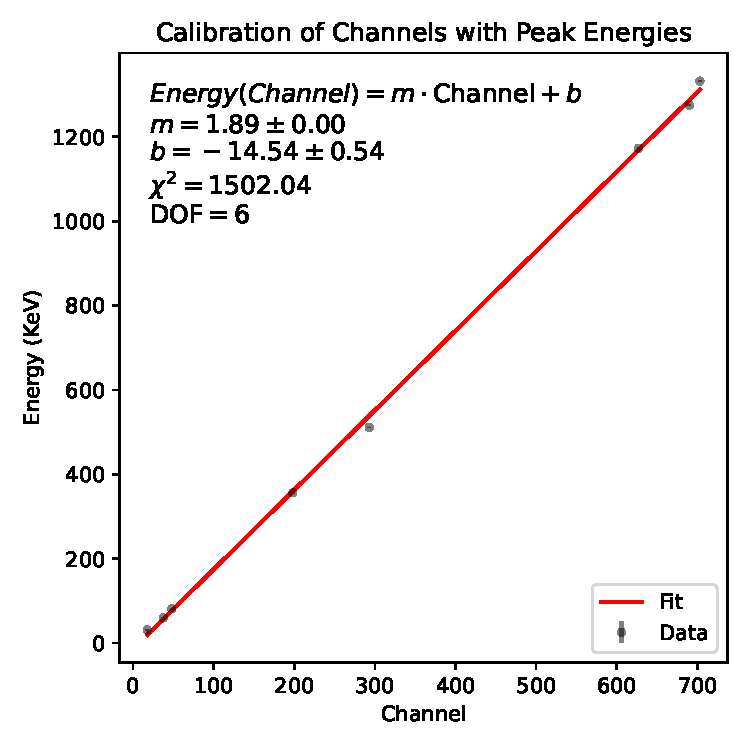
\includegraphics[width=0.5\textwidth]{experiment2/figures/calibration.pdf}
    \caption{}
    \label{fig:cs137-spectrum}
\end{figure}

In this lab we seek to evaluate the quantum mechanical model for scattering proposed by Compton. 

\begin{table}[h]
\centering
\begin{tabular}{|c | c c c c c c c |}
    \hline
    Theta (deg) & $0 \pm 1$ & $30 \pm 1$ & $45 \pm 1$ & $60 \pm 1$ & $90 \pm 1$ & $105 \pm 1$ & $120 \pm 1$ \\
    Centroid & \\
    Gain & $2$ & $2$ & $2$ & $2$ & $2$ & $2$ & $2$ \\
    \hline
    Channel \\
    \hline
\end{tabular}
\caption{Fitted and expected linear attenuation coefficients for various energy levels.}
\label{table:1}
\end{table}

\end{document}